\documentclass[a4paper]{instrumentacao}

\usepackage{etoolbox}

\newtoggle{attachments}
\toggletrue{attachments}

\graphicspath{
	{../Resources/Images/}
	{../Resources/Mathematica/images/}
	{../Resources/MATLAB/images/}
}

\title{???}
\author{Rogiel Sulzbach \and Rodrigo de Castro Silveira}
\startdate{???}
\finishdate{???}
\emails{
	\emailaddress{R.J.S.}{rogiel@rogiel.com},
	\emailaddress{R.C.S.}{csilveira.rodrigo@gmail.com}
}

\resume{}
\abstract{} 
\keywords{}
\institute{}

\headertext{Extensometria}

\begin{document}
\maketitle

\todo{Tarefa no Laboratório: selecionar duas células disponibilizadas no laboratório de 
instrumentação (01 célula de carga não comercial do tipo viga engastada e 01 célula de carga comercial do tipo viga engastada – (para a célula de carga comercial ver Figuras 17 ou 18 e Tabelas 8 ou 9 – selecionar apenas 01 modelo da célula comercial)). Desenvolver usando o SolidWorks o correspondente modelo virtual e determinar o comportamento estático e dinâmico do modelo virtual para cada uma das células de carga. Observações: material da célula de carga não comercial é alumínio naval (várias células de carga, não comerciais, estão deformadas, mas mesmo assim trabalhar com as mesmas e suas não idealidades) e da célula comercial é Alumínio Anodizado. Limite de carga: 400g para a célula de carga não comercial e 5kg para a célula de carga comercial!}
\todo{Tarefa no Laboratório: selecionar a célula de carga (ver Figuras 19 e 20) disponibilizada no Laboratório de Instrumentação. Desenvolver usando o SolidWorks o correspondente modelo virtual e determinar o comportamento estático e dinâmico do modelo virtual. Observações: material da célula de carga é o aço inox AISI304 e a carga limite no eixo principal é de 250N. }
\todo{Tarefa no Laboratório: usando as duas células de carga (01 não comercial e outra comercial) do item i desenvolver um condicionador de sinais para cada célula de carga. Considerar a margem de carregamento mecânico utilizado na simulação (compatível com os limites de carga fornecidos no item i). Projetar e apresentar a Cadeia de Medida desenvolvida para cada célula de carga. Obter formas de onda no LabVIEW apresentando gráficos com escala e eixos adequados a aplicação. Sugestão: analisar a revisão bibliográfica deste laboratório para auxiliar o grupo no melhor projeto.}
\todo{Tarefa no Laboratório: considerando-se a célula de carga não comercial - do item anterior (com condicionador incluso): faça uma análise sobre o efeito da variação de temperatura nestas vigas. Como sugestão aplicar rapidamente uma fonte de calor na extremidade livre da célula de carga – LONGE DO EXTENSÔMETRO e verificar o comportamento de sua ponte. Sugestão: realize a aquisição destes dados.}
\todo{Drift (deriva): remover o maior peso padrão utilizado na calibração estática e imediatamente registrar Vo (registrar durante 5 minutos);}
\todo{Reprodução dos Valores: recolocar o maior peso padrão e registrar Vo. Remover o peso e imediatamente registrar Vo; }
\todo{Efeito do aquecimento: suavemente aquecer o topo da barra (sem carga). Registrar qualquer mudança em Vo enquanto aquece (não aquecer mais do que 10C e nunca sobre o strain-gage). Estimar a variação da temperatura. Aquecer a parte de baixo da barra e repetir os procedimentos anteriores deste item. Repetir novamente, porém aquecendo o topo e a parte de baixo da barra (ao mesmo tempo).}


\todo{Tarefa no Laboratório: considerando-se apenas a célula de carga não comercial (do item anterior): realizar o teste do impacto para determinar a frequência de ressonância dessa estrutura. Neste tipo de ensaio o padrão (e o correto) é utilizar um acelerômetro adequado, porém neste laboratório irão utilizar o(s) próprio(s) extensômetro(s). Utilizar uma placa de aquisição de dados (verificar se a entrada desta placa não será danificada pelo condicionador de vocês). Adquirir sinais no tempo durante a realização deste ensaio. Depois determinar a FFT deste sinal e discutir os resultados obtidos. Comparar com os dados da simulação dinâmica da célula de carga.}
\todo{Tarefa no Laboratório: considerando-se o torquímetro disponibilizado, no laboratório de instrumentação, projetar a cadeia de medição e o correspondente condicionamento. Apresentar seus resultados e comparar com os aspectos teóricos apresentados neste relatório.}

\todo{Faça uma comparação dos dados experimentais e/ou dos dados simulados e deste modelo. Discutir as suas diferenças.}

\todo{ladainha dos circuitos, de novo}

\chapter{Introdução}

Nesta atividade de relatório foram feitas várias atividades de laboratório utilizando sensores do tipo extesômetro. Um extensômetro é um sensor resistivo cuja resistência elétrica varia com a deformação mecânica do sensor. A Figura \ref{fig:intro-extensometro} apresenta um extensômetro do tipo grade:

\begin{figure}[H]
\center
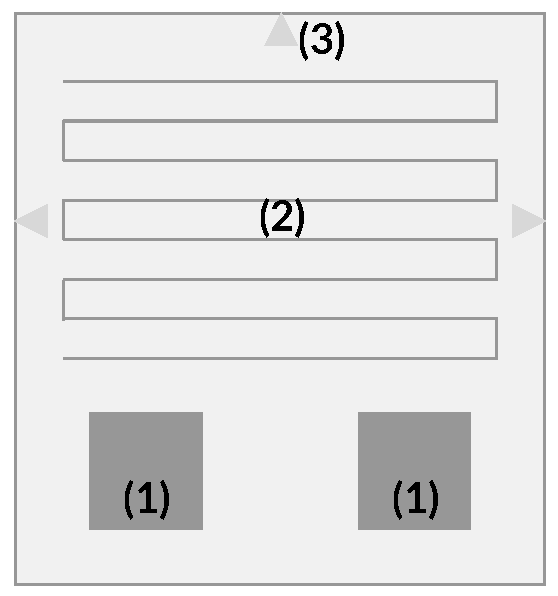
\includegraphics[width=0.5\textwidth]{ExtensometroGrade.pdf}
\caption{Desenho simplificado de um extensômetro do tipo grade}
\label{fig:intro-extensometro}
\end{figure}

\noindent onde (1) representa os \textit{pads} de conexão elétrica do sensor, (2) é a grade do sensor e (3) são os indicadores de alinhamento do sensor.

Conforme apresentado na Figura \ref{fig:intro-extensometro} a grade do sensor (2) é composta por um material condutor com uma resistência elétrica característica. Uma vez que o sensor esteja cimentado (colado) sobre uma superfície deformações na superfície se propagam como deformação do sensor que deformam a grade. Deformações na grade causam pequenas alterações (na ordem de $10^{-6} \Omega$) na resistência elétrica do sensor. Com um circuito elétrico de condicionamento adequado, estas pequenas variações de resistência elétrica do sensor podem ser medidas e quantificadas em valores de deformação mecânica.

Os indicadores de alinhamento do sensor (3) conforme apresentados na figura \ref{fig:intro-extensometro}, indicam o ponto de maior sensibilidade do sensor, isto é, onde há a maior variação de resistência elétrica para uma mesma deformação.

O extensômetro pode ser modelado matematicamente de forma simplificada pela Equação \ref{eq:intro-extensometro}:

\begin{equation}
	\frac{\Delta R}{R_0} = k \frac{\Delta l}{l_0} = k\epsilon
	\label {eq:intro-extensometro}
\end{equation}

\noindent onde $\Delta R/R_0$ é a variação relativa de resistência elétrica do sensor referente ao seu valor inicial de repouso (ou nominal) $R_0$, $\Delta l/l_0$ é a deformação mecânica relativa do sensor referente ao seu valor inicial de repouso (ou nominal) $l_0$ também definida como $\epsilon$ e $k$ é uma constante que define a relação entre variação de resistência elétrica e deformação do sensor.

Dessa forma, é possível relacionar a deformação mecânica da grade do sensor com a variação de resistência elétrica do sensor. Como a variação de resistência elétrica é muito baixa (ordem de $10^{-6}$) para que seja possível medir esta variação é necessário que se utilize um circuito de condicionamento de qualidade. Uma topologia muito comum é a utilização da ponte de Wheatstone, que são origem à 3 montagens comuns com extensômetros: 1/4 de ponte, meia ponte e a ponte completa.

\chapter{Metodologia Experimental}
Nestes experimentos de laboratório foi utilizado o software Wolfram Mathematica 10.4.0 da Wolfram Research, Inc. para realizar todos os cálculos no computador utilizando precisão do tipo MachinePrecision\cite{mathematica-numerial-precision} onde a precisão dos números de ponto flutuante respeitam os critérios impostos pelo processador (64 bits, precisão dupla) que implementam o padrão IEEE de ponto flutuante, possuem um "Épsilon de Máquina", o menor valor que somado a 1 retorna um valor diferente de 1, isto é, não causa arredondamento \cite{wikipedia-epsilon}, de $2^{-52}$, ou seja, na ordem de $10^{-16}$ e podem, portanto, serem desprezados perante a resolução de todos os outros instrumentos utilizados no experimento. Adicionalmente, quando possível, os cálculos foram realizados de forma simbólica com substituição numérica no final. Os scripts utilizados para cálculo estão anexados ao fim do documento, na Página \pageref{ch:attachments}.

Para a realização das simulações mecânicas, o SOLIDWORKS versão 2016 desenvolvido pela Dassault Systèmes SolidWorks Corp.

\section{Célula de força comercial}

Neste experimento foi levantada a função de transferência experimental para uma viga engastada utilizando uma célula de força comercial \todo{marca e outros detalhes da célula}.

Na Figura \ref{fig:celula-comercial-circuito} está apresentado o esquemático elétrico de uma ponte de Wheatstone:

\begin{figure}[H]
\center
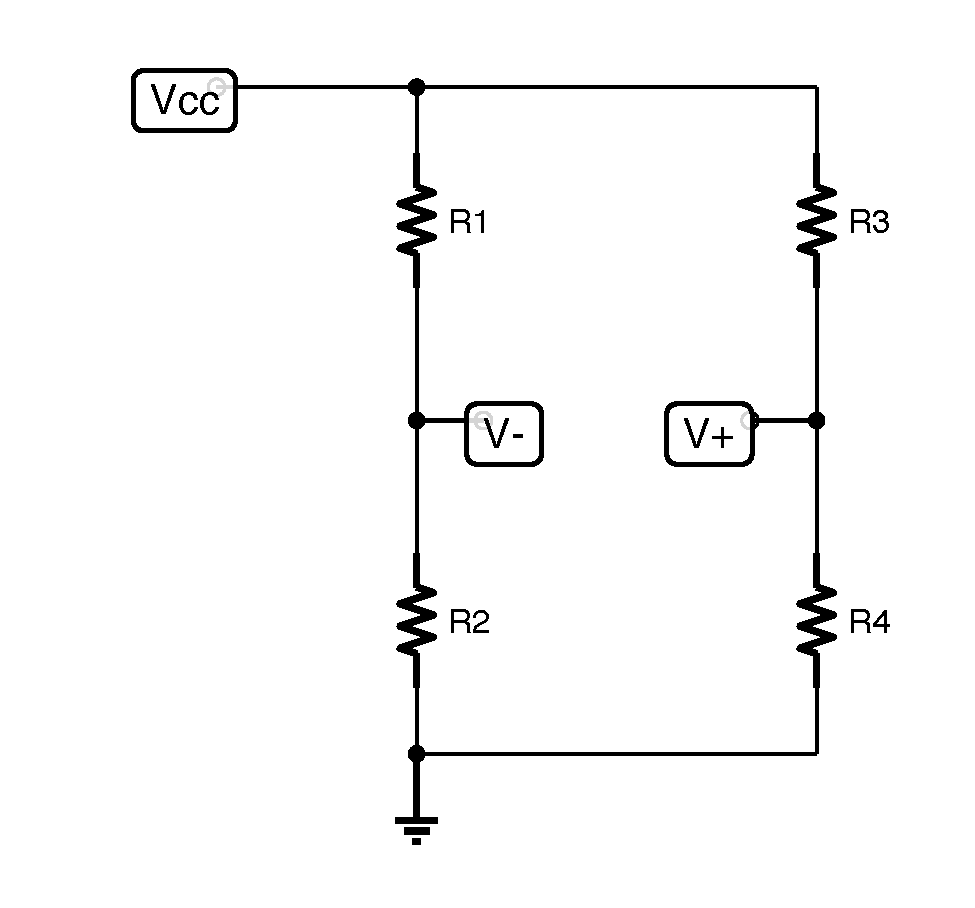
\includegraphics[width=\textwidth]{Wheatstone.pdf}
\caption{Esquemático elétrico de uma ponte de Wheatstone genérica.}
\label{fig:celula-comercial-circuito}
\end{figure}

\noindent onde os resistores $R_1$, $R_2$, $R_3$ e $R_4$ são valores de resistência elétrica que determinam o comportamento de ponte, $V_-$ e $V_+$ são os nós de saída da ponte medidos em tensão elétrica e $V_{cc}$ é a tensão elétrica de alimentação da ponte.

A função de transferência da ponte de Wheatstone proposta é dada conforme Equação \ref{eq:wheatstone-tf}:

\begin{equation}
	V_o = V_+ - V_- = \left(\dfrac{R_4}{R_4 + R_3} - \dfrac{R_2}{R_1 + R_2}\right)V_{cc}
	\label{eq:wheatstone-tf}
\end{equation}

Considerando que as condições das Equações \ref{eq:celula-comercial-cond1} e \ref{eq:celula-comercial-cond2} são válidas, então a ponte é dita estar "em equilíbrio", isto é, a saída de tensão elétrica entre $V_-$ e $V_+$ é de $OV$.

\begin{eqnarray}
	R_1 = R_4 \label{eq:celula-comercial-cond1} \\
	R_2 = R_3 \label{eq:celula-comercial-cond2}
\end{eqnarray} 

Qualquer pequena variação de resistência elétrica em qualquer um dos resistores da Figura \ref{fig:celula-comercial-circuito} que violem as condições da Equação \ref{eq:celula-comercial-cond1} e \ref{eq:celula-comercial-cond2} incorre no desequilíbrio da ponte que pode ser medido utilizando a saída em tensão elétrica.

Com isto, a ponte pode ser utilizada como circuito de condicionamento para um sistema de medição de deformação mecânica de um corpo. Na Figura \ref{fig:celula-comercial-esquema-fisico} está apresentado um esquemático físico da célula de carga comercial utilizada:

\begin{figure}[H]
\center
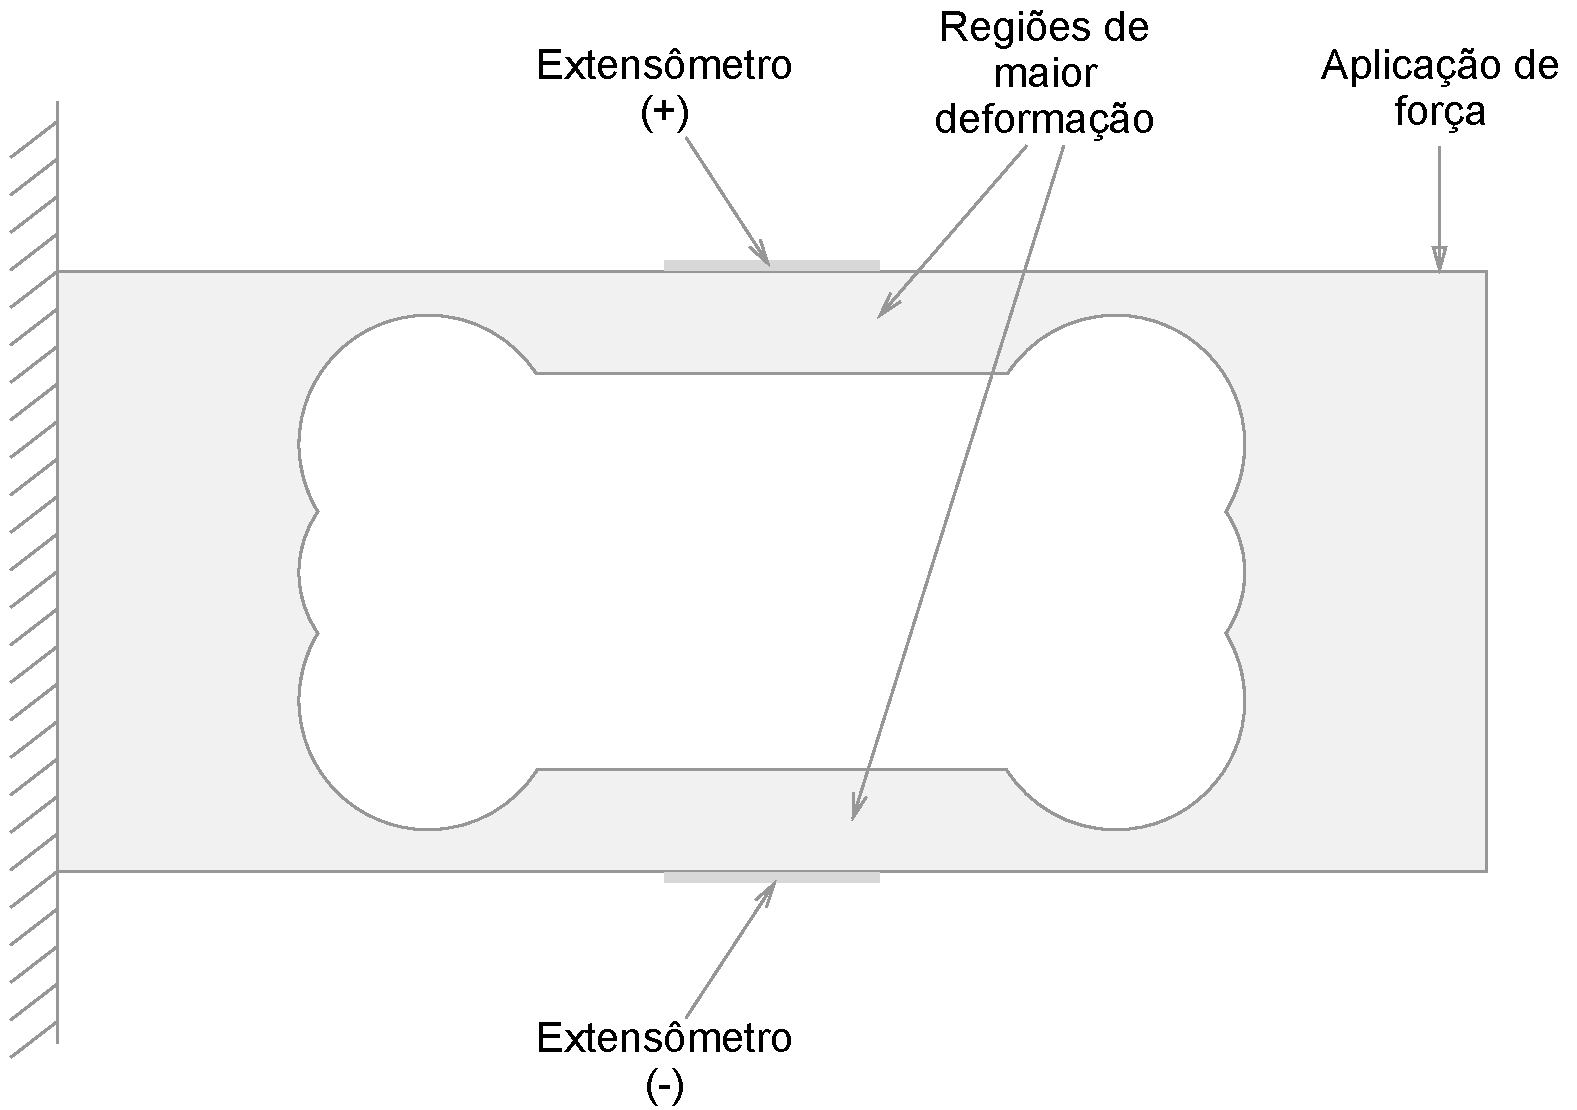
\includegraphics[width=\textwidth]{CelulaComercial.pdf}
\caption{Esquemático da construção mecânica da célula de carga comercial utilizada no experimento.}
\label{fig:celula-comercial-esquema-fisico}
\end{figure}

\noindent onde o extensômetro $(+)$ indica uma deformação positiva (alongamento) e o extensômetro $(-)$ indica uma deformação negativa (compressão).

Portanto, é possível utilizar esta construção como forma de medir deformações que a viga proposta esteja submetida. É comum utilizar 3 formas distintas de medição utilizando extesômetros e a ponte de Wheatstone.

\todo{continuar}

\section{Célula de força não-comercial}

A célula de força não comercial utilizada possui a configuração dada na Figura \ref{fig:celula-nao-comercial-desenho}:

\begin{figure}[H]
\center
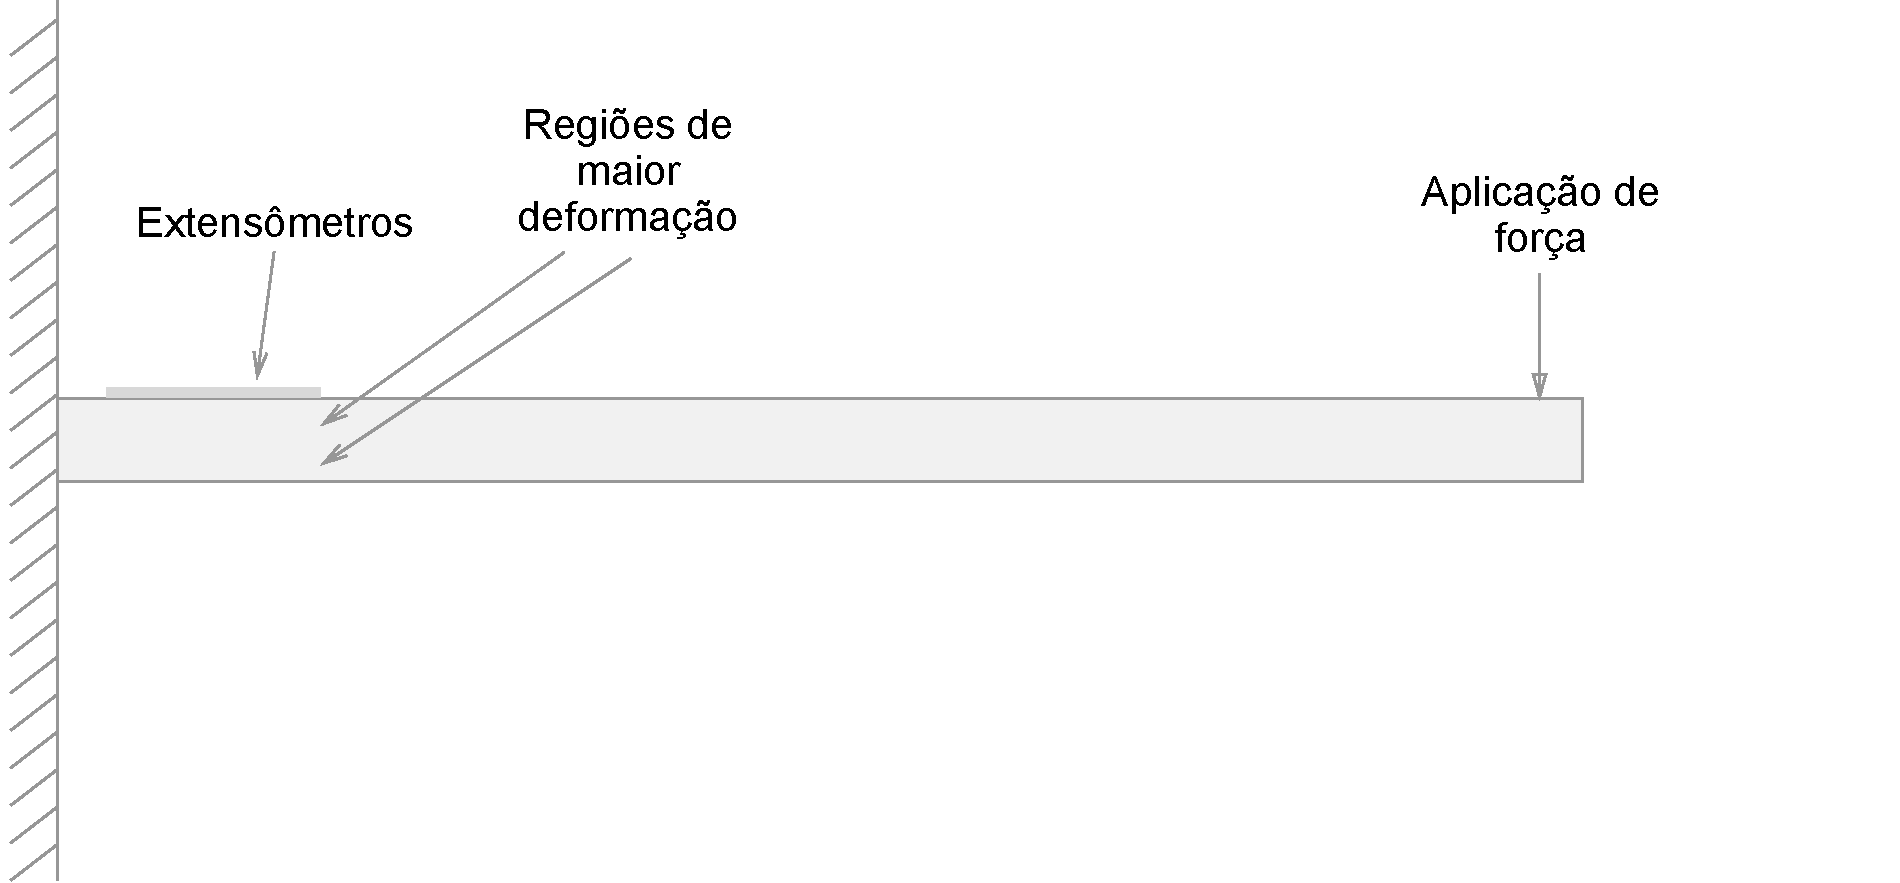
\includegraphics[width=\textwidth]{CelulaNaoComercial.pdf}
\caption{Esquemático da construção mecânica da célula de carga não-comercial utilizada no experimento.}
\label{fig:celula-nao-comercial-desenho}
\end{figure}

\noindent onde o extensômetro $(+)$ indica uma deformação positiva (alongamento) e o extensômetro $(-)$ indica uma deformação negativa (compressão). É importante observar que a célula possuía um extensômetro na parte superior (próximo à base de suporte) e outro extensômetro na mesma posição, mas na face inferior da barra. Em termos prático, isto significa que para uma mesma deformação, o variação de resistência elétrica em ambos os extensometros é idêntica em módulo, mas com diferente sinal. Este comportamento é importante pois espera-se que a saída da ponte de Wheatstone fique constante com o aquecimento da barra, fato que não aconteceria caso fosse utilizada a mesma face da ponte para a colagem dos extensômetros.

Ao contrário da célula comercial, esta nao possui a ponte pré-calibrada e, portanto, se fez necessário que a ponte fosse calibrada e ajustada para obter o resultado desejado. De acordo com a especificação dos extensômetros (modelos e fabricantes não estavam explícitos sobre a construção, logo, não foi possível comparar com os valores fornecidos pelo fabricante). Havia, contudo, uma marcação indicando o valor de resistência nominal do extensômetro.

Considerando que a resistência elétrica nominal da célula de carga quando em repouso seja de $350 \Omega$ com incerteza desconhecida, é possível calcular os resistores para os demais braços da ponte de Wheatstone. A Figura \ref{fig:celula-nao-comercial-ponte}

\begin{figure}[H]
\center
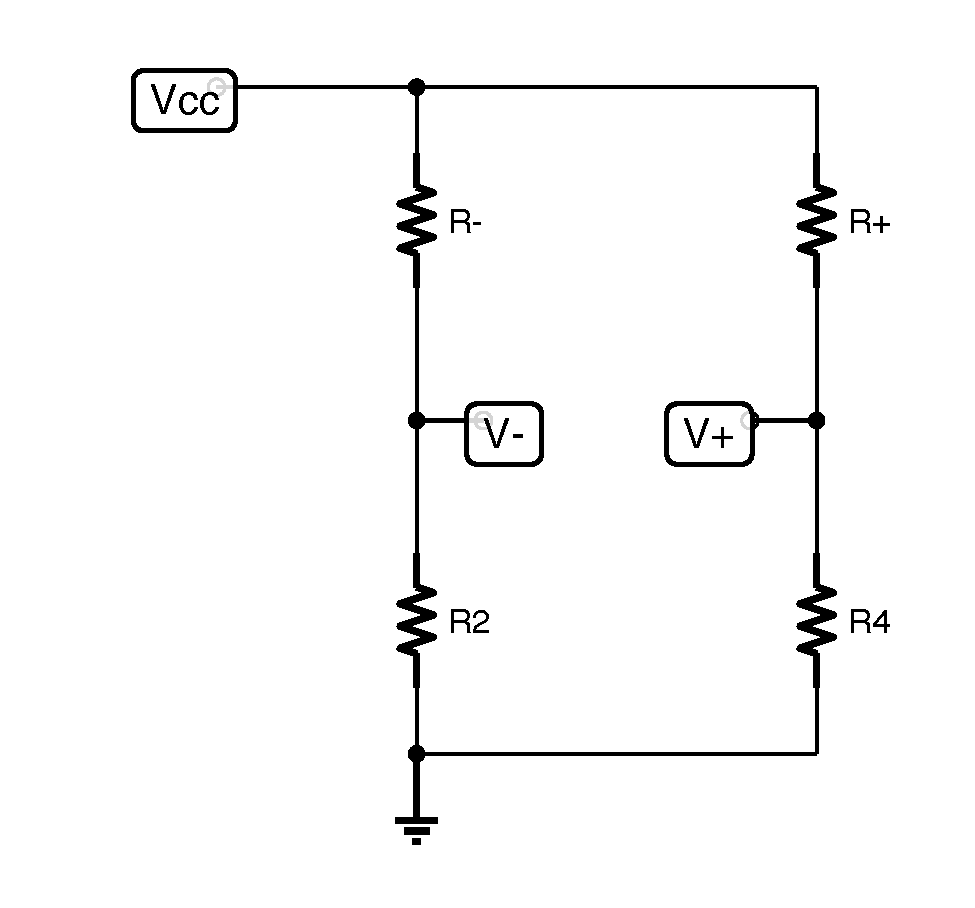
\includegraphics[width=\textwidth]{WheatstoneNaoComercial.pdf}
\caption{Esquemático elétrico da ponte de Wheatstone para a célula de carga não-comercial. O modelo escolhido foi utilizar uma meia-ponte, com variação positiva e outra negativa.}
\label{fig:celula-nao-comercial-ponte}
\end{figure}

\noindent onde os resistores $R_2$ e $R_4$ são resistores cujo valor deve ser o mais próximo possível do valor nominal dos extensômetros da ponte e $R+$ e $R-$ são os extensômetros com variação, respectivamente, positiva e negativa, de resistência elétrica em função da deformação da barra.

\subsection{Modelo computacional}
A fim de realizar uma validação computacional dos resultados, foi desenvolvido um modelo computacional para a célula de força não-comercial no software SOLIDWORKS 2016 x64 e realizada utilizando o método FFEPlus com a opção de \textit{large displacement} desativada.

Na simulação de análise estática da célula, foi aplicada uma força de ??? N \todo{quanto?} sobre o furo presente na barra. A Figura \ref{fig:celula-nao-comercial-solid-modelo} apresenta o modelo 3D desenvolvido no software:

\begin{figure}[H]
\center
%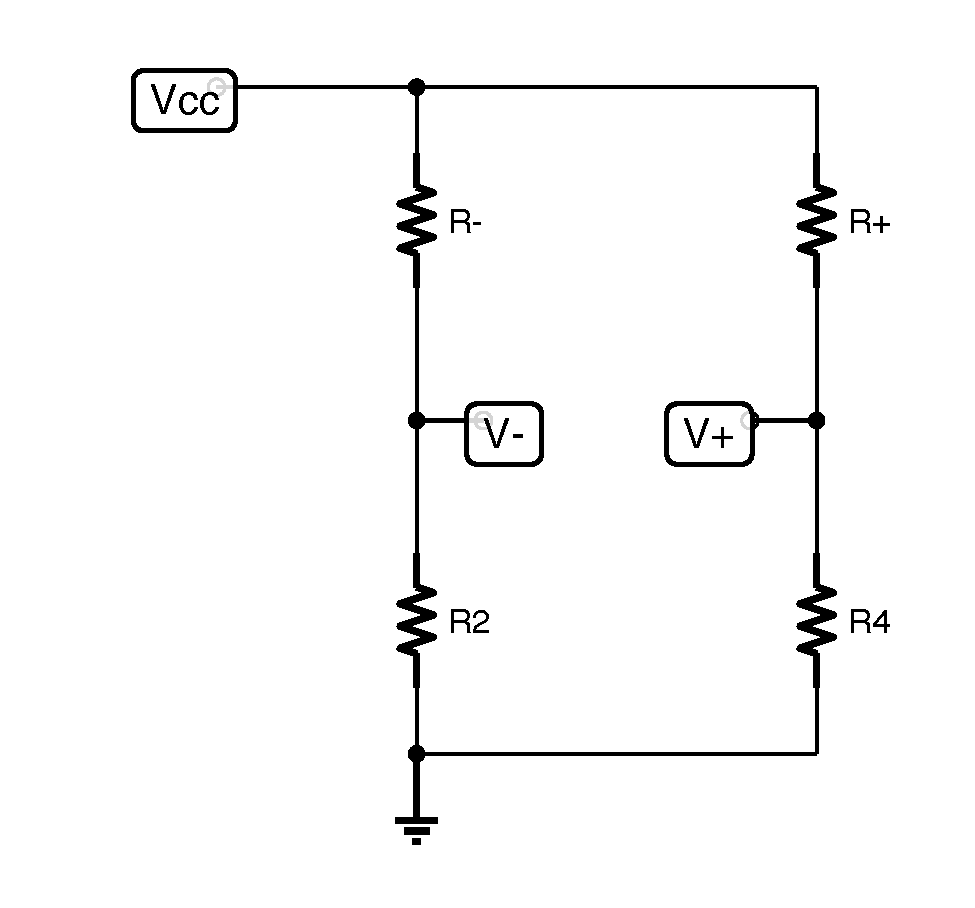
\includegraphics[width=\textwidth]{WheatstoneNaoComercial.pdf}
...
\caption{Modelo 3D utilizado para a simulação da célula de força não-comercial no SOLIDWORKS.}
\label{fig:celula-nao-comercial-solid-modelo}
\end{figure}
\todo{figura solid}

\noindent onde a superfície de aplicação da força é o orifício utilizado para exercer as forças durante a execução do experimento no laboratório.

Nesta simulação foi possível estimar a deformação da barra para os valores de 2N, 4N, 6N, 8N e 10N que correspondem, aproximadamente aos pesos das massas de 200g, 400g, 600g, 800g e 1kg (considerando que a aceleração local da gravidade $g$ é dada, aproximadamente, por $10 m/s^2$.

A fim de determinar a frequência fundamental da vibração do sistema, foi realizada uma simulação dinâmica de frequência do sistema. Nesta simulação a frequência fundamental de vibração do sistema foi extraída e validada com o experimento em que uma batida é feita na barra e pela vibração medida pelo extensômetro é possível estimar a frequência fundamental de vibração do sistema.

\section{Torquímetro}


\chapter{Resultados e Discussões}

\chapter{Conclusões}

\newpage

\begin{thebibliography}{9}
\bibitem{mathematica-numerial-precision} \url{https://reference.wolfram.com/language/tutorial/NumericalPrecision.html}, acessado em 26 de abril de 2016
\bibitem{wikipedia-epsilon} \url{https://en.wikipedia.org/wiki/Machine_epsilon}, acessado em 26 de abril de 2016
\bibitem{livro-texto}  Balbinot, Alexandre; Brusamarello, Valner J., Instrumentação e Fundamentos de Medida - Vol.1 - 2ª Ed. Rio de Janeiro: LTC, 2014.
\bibitem{daq-specifications} NI USB-6009 -- DEVICE SPECIFICATIONS, \url{http://www.ni.com/pdf/manuals/375296a.pdf}, acessado em 3 de maio de 2016
\bibitem{daq-user-guide} NI USB-6009 -- USER GUIDE, \url{http://www.ni.com/pdf/manuals/371303n.pdf}, acessado em 3 de maio de 2016
\bibitem{datasheet-lm7805} Datasheet oferecido pelo fabricante do regulador de tensão LM7805CV, disponível em \url{http://www.datasheetlib.com/datasheet/221840/l7805cv_stmicroelectronics.html}.
\bibitem{datasheet-ina126} Datasheet oferecido pelo fabricante amplificador de instrumentação INA126, disponível em \url{http://www.ti.com/lit/ds/symlink/ina126.pdf}.

\end{thebibliography}

\iftoggle{attachments}{
	\chapter*{Anexos}
	\label{ch:attachments}
	\section{Mathematica}
	
}

\end{document}
